\chapter{T�tulo cap�tulo 2}

\section{Estado del arte}

Texto y m�s texto... La figura \ref{fig01} es un ejemplo de como insertar im�genes en la tesis


\begin{figure}[htpb]
	\center
	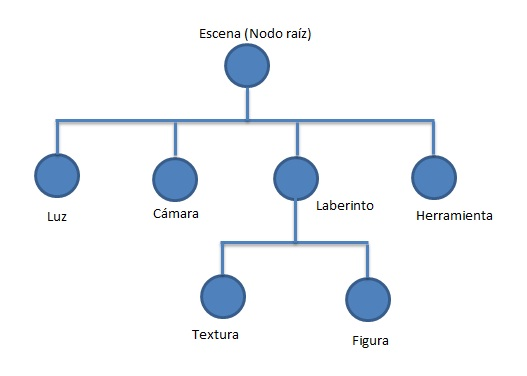
\includegraphics[width=11cm,height=8cm]{imag//nombredelaimagen.jpg}\\
	\caption{T�tulo de la imagen.}\label{fig01}
	\endcenter
\end{figure}


\subsection{Uso de llaves}
Es un ejemplo de como usar los diagramas de llaves
\begin{displaymath}
Tema Principal\left\lbrace
\begin{array}{lcr}
subtema1\\
subtema2 \left\lbrace 
	\begin{array}{lcr} 
		uno\\
		dos 
	\end{array} \right.\\
subtema3\\
ultimosubtema
\end{array} \right.
\end{displaymath} 

\section{Dos Figuras}

Ejemplo de insertar dos figuras (hacerlo bajo su propio riesgo... no muy recomendado)

\begin{figure}[htbp]
	\begin{minipage}{7cm}
		\centerline{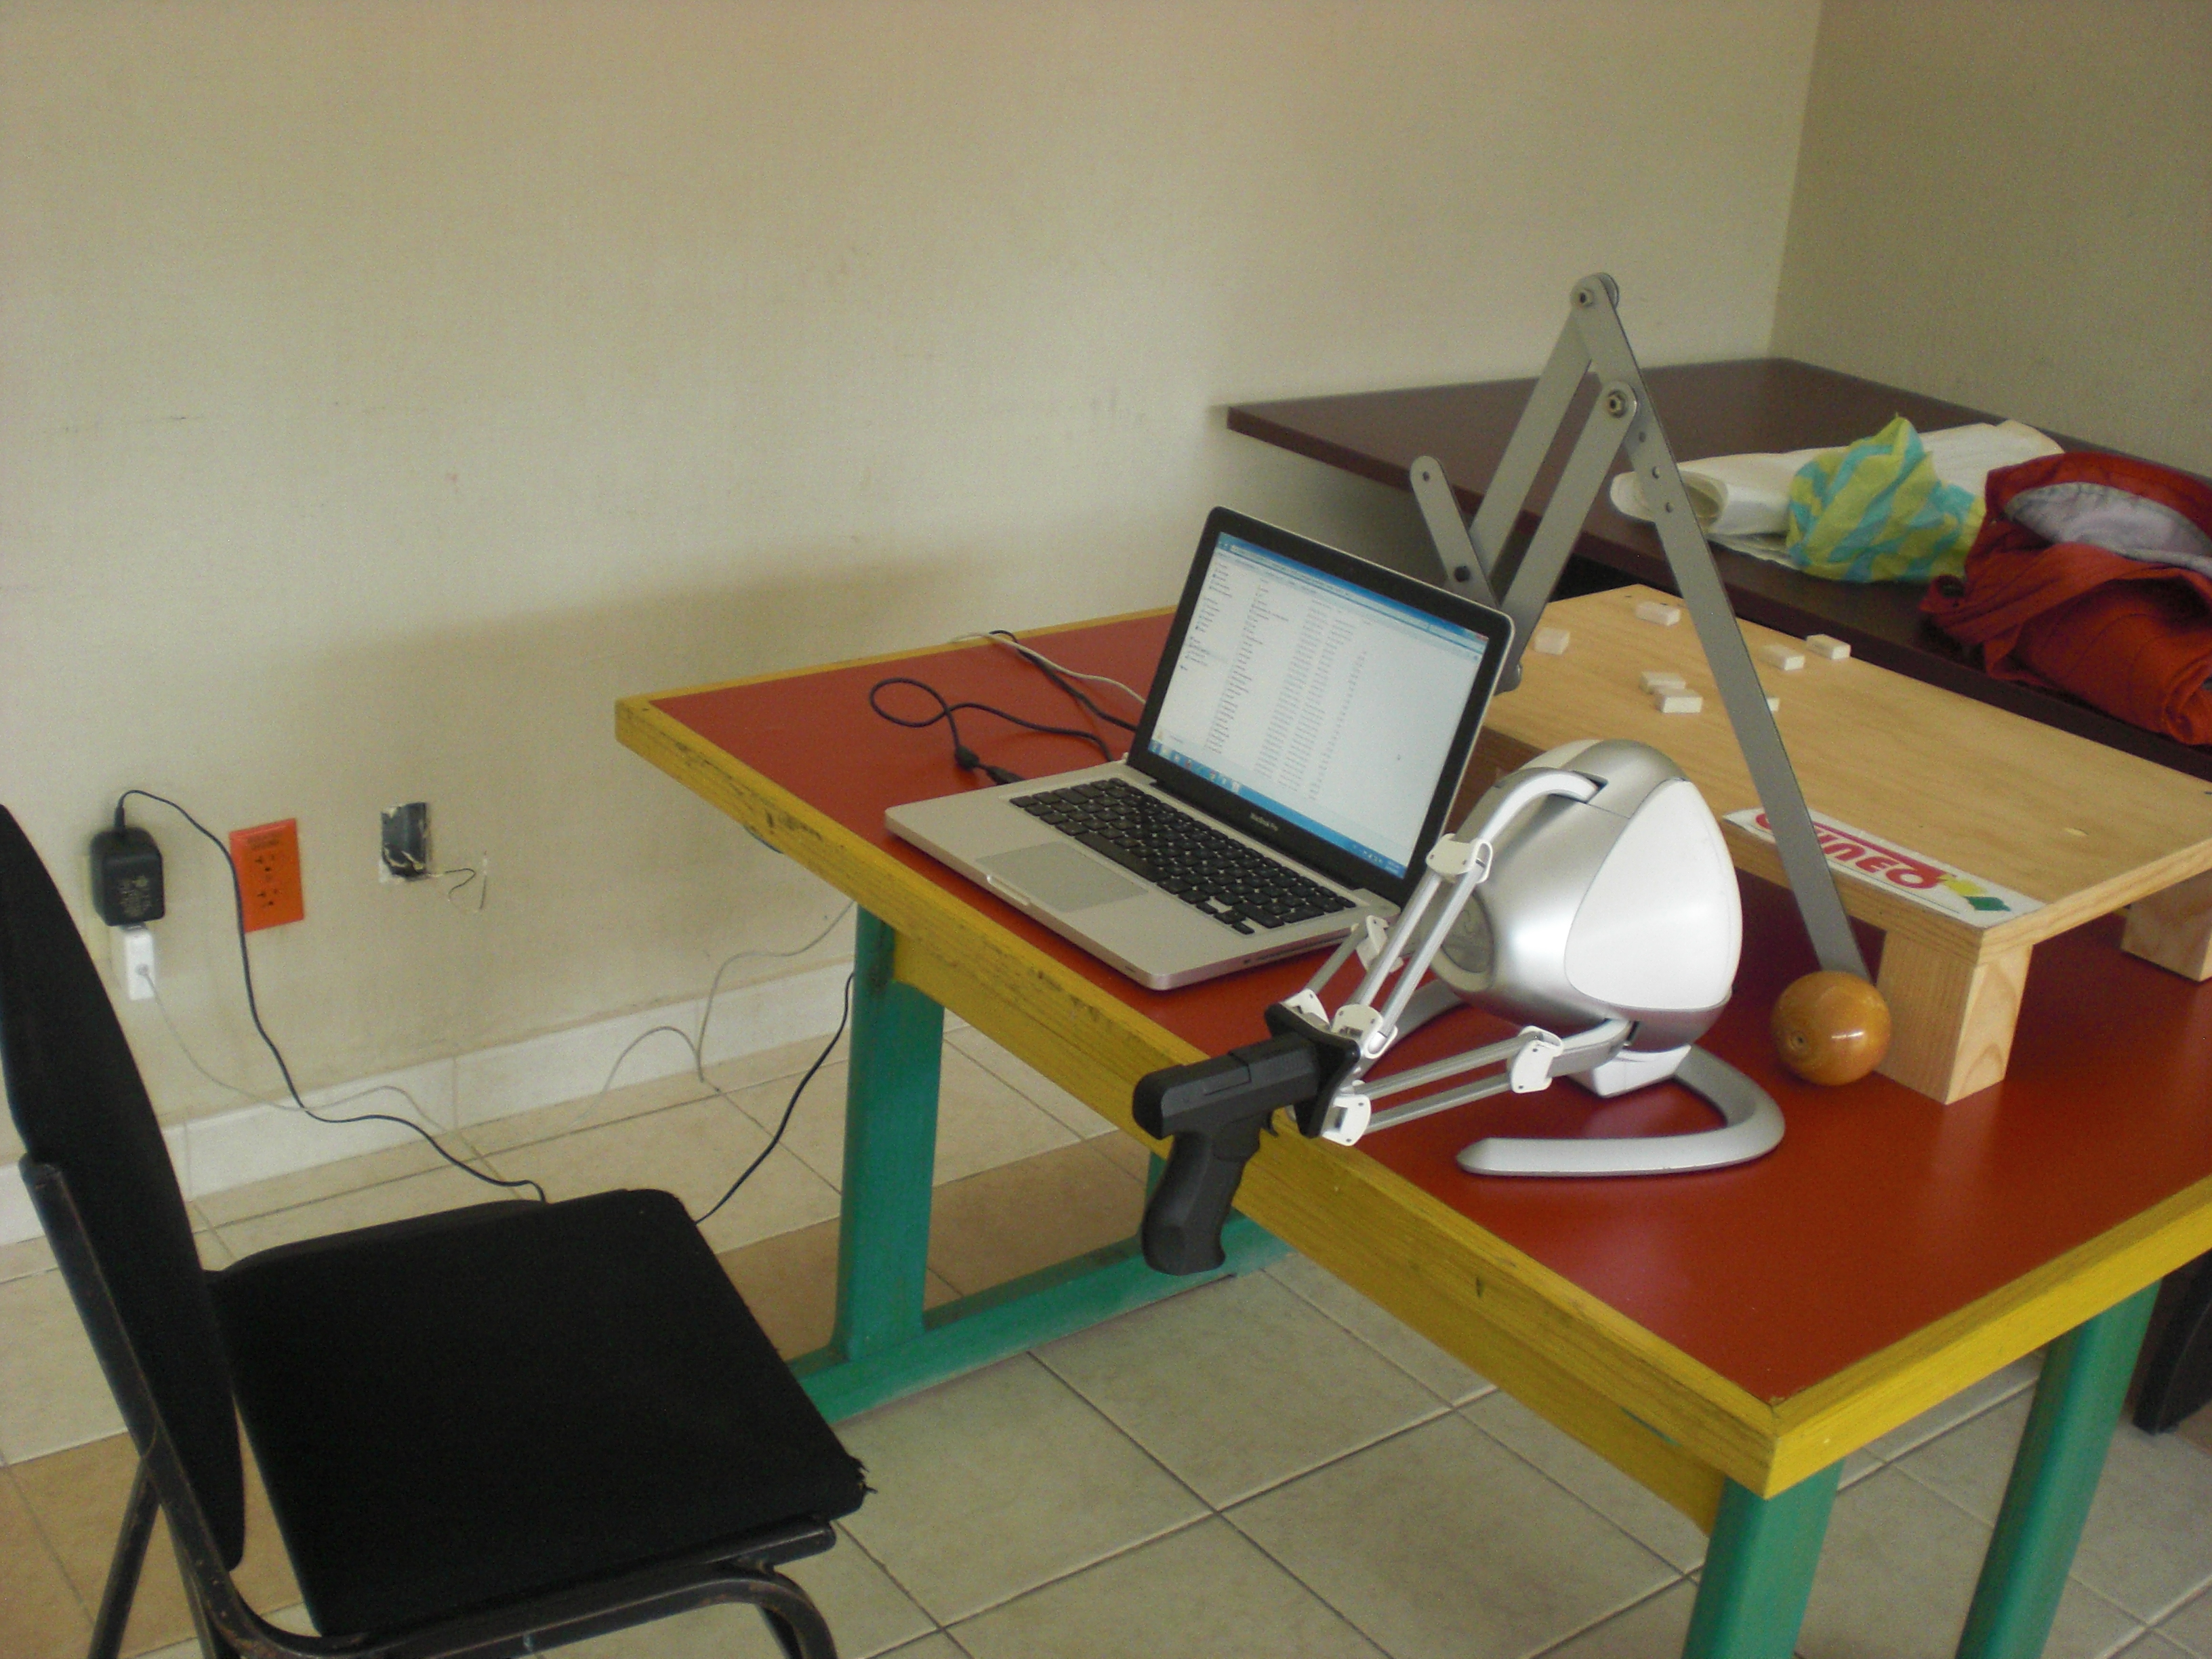
\includegraphics[height=5cm,width=7cm,angle=0]{imag//cree//Izquierda.jpg}}
		\vspace{0.5cm}
		\caption{T�tulo imagen izquierda.}\label{figIz}
	\end{minipage}\hspace{0.8cm}
	\begin{minipage}{7cm}
		\centerline{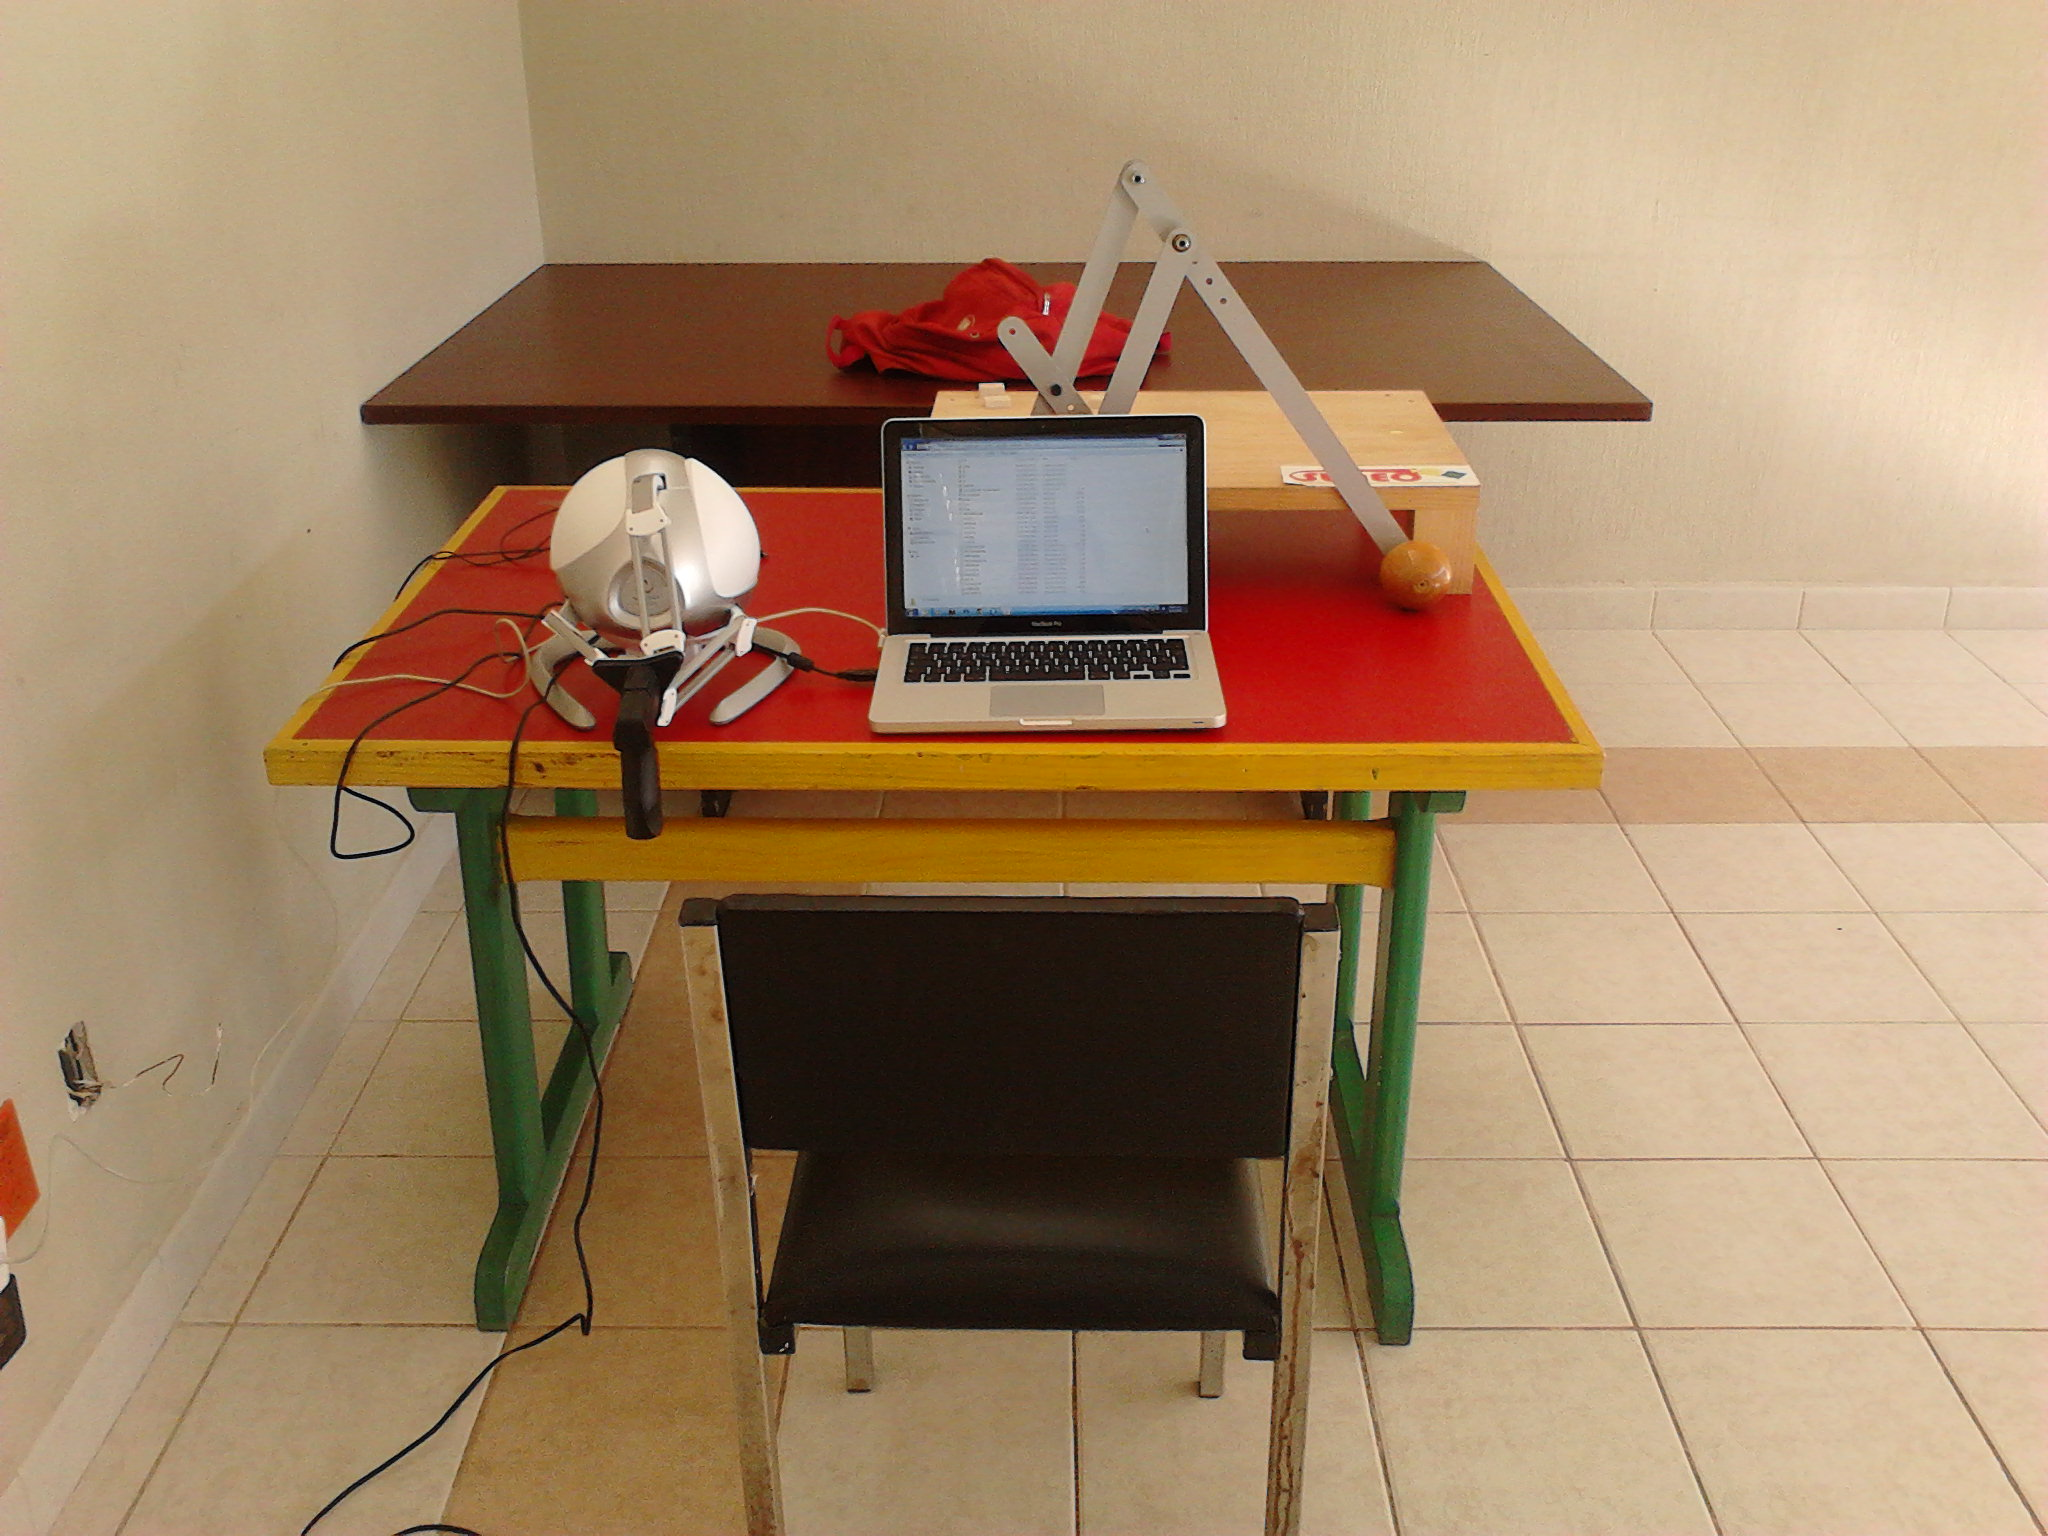
\includegraphics[height=5cm,width=7cm,angle=0]{imag//cree//Derecha.jpg}}
		\vspace{0.5cm}
		\caption{T�tulo imagen derecha.}\label{figDe}
	\end{minipage}
\end{figure}

A continuaci�n se muestra la forma de realizar un listado...

\begin{enumerate}
	\item Item 1
	\item Item 2
	\item Item 3
\end{enumerate}

Otra forma de enlistar..

\begin{enumerate}
	\item[a)] Item a
	\item[b)] Item b
	\item[c)] Item c
\end{enumerate}

Otro estilo.. 

\begin{itemize}
	\item Item a.1
	\item Item a.2
	\item Item a.3
\end{itemize}

\subsection{Ejemplos de Tablas}

\subsubsection{Insertar tabla a dos columnas}
Como se inserta la tabla \ref{tabla1} 
\begin{table}[h]
	\caption{Descripci�n de la tabla}\label{tabla1}
	\vspace{-0.5cm}
	\begin{center}
		\begin{tabular}{|p{5cm}|p{5cm}|}
			\hline
			Campo11 & Campo12 \\
			\hline
			Campo21 & Campo22\\
			\hline
			Campo31 & Campo32 \\
			\hline
		\end{tabular}
	\end{center}
\end{table}

\subsubsection{Insertar tabla a m�s columnas}

Como se inserta la tabla \ref{tabla2}

\begin{table}[htpb]
	\caption{Descripci�n de la tabla}\label{tabla2}
	\vspace{-0.5cm}
	\begin{center}
		\begin{tabular}{|p{3cm}|p{3cm}|p{3cm}|p{3cm}|}
			\hline
			Campo11 & Campo12 & Campo13 & Campo14 \\ \hline
			Campo21 & Campo22 & Campo23 & Campo24 \\ \hline
			Campo31 & Campo32 & Campo33 & Campo34 \\ \hline
		\end{tabular}
	\end{center}
\end{table}


\subsection{Otros formatos}

Las ecuaciones del pant�grafo est�n dadas por las ecuaciones:

\begin{equation}\label{eq1}
\lambda*AB=AE
\end{equation}
\begin{equation}\label{eq2}
\lambda*ED=EF
\end{equation}
\begin{equation}\label{eq3}
\lambda*AC=AF
\end{equation}
Donde $\lambda$ representa la escala de reproducci�n tal  que $\lambda>0$, y $\lambda\neq1$
determinando as�  que para el caso de la plataforma $\lambda=2$ considerando agregar 5cm de m�s al segmento EF
para colocar el sujetador final \cite{capitulo32}.


Para determinar el grupo de control se elabor� un cuestionario que fue aplicado a una muestra de poblaci�n de forma aleatoria (uso de verbatim).
\begin{verbatim}
Entrevista n�mero: _____________________

Edad: ______    Escolaridad: _______________
Estado civil: _____________
Ocupaci�n: ________________________________________________
La siguiente encuesta tiene como fin el establecer un grupo
de control  por lo que sus respuestas ser�n tratadas de for-
ma confidencial y la informaci�n que nos proporcione ser�
exclusivamente para la investigaci�n llevada a cabo.
Por tal motivo pedimos contestar con la mayor sinceridad
posible.

1.- �Usted consume bebidas alcoh�licas?
Si ____                         No_____
Si su respuesta fue "No", omita la siguiente pregunta
1.1	�Con que frecuencia usted consume bebidas alcoh�licas?
a)	Frecuentemente	b) a veces	c) solo en fiestas u ocasionalmente
2.- �sufre usted de hipertensi�n?
Si ____		         No____
3.- �Es usted zurdo o diestro?
____ Zurdo	        ___Diestro
4.- �Ha sufrido alg�n tipo de lesi�n en el brazo o en las manos (fracturas)?
SI____		        No_____
5.- �Ha tenido alg�n antecedente de par�lisis?
S�____		       No______
6.- �Ha sufrido ataques de epilepsia?
S�______		      No_____
7.- �Padece de artritis reumatoide?
S�___ 			No____
\end{verbatim}


Ejemplo de la codificaci�n de un algoritmo en C. Algoritmo Runge Kutta

\begin{lstlisting}

double RKS(double a)
{
double h, k1, k2, k4;

h=0.001;
k1=(a);
k2=(a+h/2.0);
k4=(a+h);
return (h*(k1+4*k2+k4)/6.0);

}
cVector3d RK(cVector3d t){
cVector3d s(RKS(t.x),RKS(t.y),RKS(t.z));
return s;
}
\end{lstlisting}
